\documentclass{article}
\usepackage[utf8]{inputenc}
\usepackage{amsmath}
\usepackage{verbatim}
\usepackage{graphicx}
\usepackage{array}
\setlength{\extrarowheight}{.5ex}
\usepackage{amssymb}
\usepackage{graphicx}
\graphicspath{./}
\usepackage[margin=0.5in]{geometry}

\makeatletter
\newcommand*{\shifttext}[2]{%
  \settowidth{\@tempdima}{#2}%
  \makebox[\@tempdima]{\hspace*{#1}#2}%
}
\newcommand{\hella}{\bBigg@{4}}
\newcommand{\hellla}{\bBigg@{5}}
\newcommand{\indicate}{\text{I} \shifttext{-3pt}{I}}
\newcommand{\msp}{\text{ }}
\makeatother

\title{Statistical Pattern Recognition HW 6}
\author{Brandon Duderstadt}

\begin{document}
  \maketitle
  \section*{1}
    Consider a set of binary data:
    $$\vec X' = \{x_1, x_2, ..., x_{12}\}$$
    Collected from a Binomial experiment where
    \begin{enumerate}
      \item $x_{12}' = 0$
      \item $\sum_i x_i' = 9$
    \end{enumerate}
    We are interested in testing the hypothesis:
    \begin{itemize}
      \item[] $\mathbf{H_0}$: $p_0 \leq \frac{1}{2}$
      \item[] $\mathbf{H_A}$: $p_0 > \frac{1}{2}$
    \end{itemize}
    At $\alpha=.05$\\[12pt]
    The following shows that two equally reasonable approaches to the analysis of this data, one Bayesian and one Frequentist, can produce different results.

    \subsection*{Bayesian}
      An uninformative uniform prior for $p$ is adopted to reflect the lack of prior information known about $p$. Since all cases of the value of $p_0$ are to be considered equally for the analysis, and no outside information is known about the distribution of $p_0$, an uninformative uniform hyperprior for $p_0$ is adopted. The relevant hypothesis test is thus written:
      $$\Lambda(x) = \frac{\sup_t \{P(\vec X | p = t)P(p=t) \text{ s.t. } t \in [0, \frac{1}{2}]\}}{\sup_t \{P(\vec X | p = t)P(p=t) \text{ s.t. } t \in (\frac{1}{2}, 1]\}} < \lambda$$
      Since the priors are uniform, and thus constant:
      $$\Lambda(x) = \frac{\sup_t \{P(\vec X | p = t) \text{ s.t. } t \in [0, \frac{1}{2}]\}}{\sup_t \{P(\vec X | p = t) \text{ s.t. } t \in (\frac{1}{2}, 1]\}} < \lambda$$
      Solving now for $\lambda$:
      $$P \hella(\frac{\sup_t \{P(\vec X | p = t) \text{ s.t. } t \in [0, \frac{1}{2}]\}}{\sup_t \{P(\vec X | p = t) \text{ s.t. } t \in (\frac{1}{2}, 1]\}} < \lambda \hella | H_0 \hella) = \alpha$$
      From the law of total probability:
      $$P \hella(\frac{\sup_t \{P(\vec X | p = t) \text{ s.t. } t \in [0, \frac{1}{2}]\}}{\sup_t \{P(\vec X | p = t) \text{ s.t. } t \in (\frac{1}{2}, 1]\}} < \lambda \hella | H_0 \hella) = \int_0^{\frac{1}{2}} P \hella(\frac{\sup_t \{P(\vec X | p = t) \text{ s.t. } t \in [0, \frac{1}{2}]\}}{\sup_t \{P(\vec X | p = t) \text{ s.t. } t \in (\frac{1}{2}, 1]\}} < \lambda \hella | p_0 = k \hella)P(p_0=k) dk$$
      From the uniform hyperprior:
      $$\int_0^{\frac{1}{2}} P \hella(\frac{\sup_t \{P(\vec X | p = t) \text{ s.t. } t \in [0, \frac{1}{2}]\}}{\sup_t \{P(\vec X | p = t) \text{ s.t. } t \in (\frac{1}{2}, 1]\}} < \lambda \hella | p_0 = k \hella) dk$$
      Thus:
      $$\int_0^{\frac{1}{2}} P \hella(\frac{\sup_t \{P(\vec X | p = t) \text{ s.t. } t \in [0, \frac{1}{2}]\}}{\sup_t \{P(\vec X | p = t) \text{ s.t. } t \in (\frac{1}{2}, 1]\}} < \lambda \hella | p_0 = k \hella) dk = \alpha$$
      Under the assumption of a binomial experiment, the likelihoods are written:
      $$\int_0^{\frac{1}{2}} P \hella(\frac{\sup_t \{\binom{12}{r}t^{r}(1-t)^{12-r} \text{ s.t. } t \in [0, \frac{1}{2}]\}}{\sup_t \{\binom{12}{r}t^{r}(1-t)^{12-r} \text{ s.t. } t \in (\frac{1}{2}, 1]\}} < \lambda \hella | p_0 = k \hella) dk = \alpha$$
      Analytically, the supremums simplify to the constrained MLE's for $p_0$. This yields:
      \begin{align*}
        &\int_0^{\frac{1}{2}} P \hella(\frac{\binom{12}{r}(\min\{\frac{r}{12}, \frac{1}{2}\})^{r}(1-\min\{\frac{r}{12}, \frac{1}{2}\})^{12-r}}{\binom{12}{r}(\max\{\frac{7}{12}, \frac{r}{12}\})^{r}(1-\max\{\frac{7}{12}, \frac{r}{12}\})^{12-r}} < \lambda \hella | p_0 = k \hella) dk = \alpha\\
        &\int_0^{\frac{1}{2}} P \hella(\frac{(\min\{\frac{r}{12}, \frac{1}{2}\})^{r}(1-\min\{\frac{r}{12}, \frac{1}{2}\})^{12-r}}{(\max\{\frac{7}{12}, \frac{r}{12}\})^{r}(1-\max\{\frac{7}{12}, \frac{r}{12}\})^{12-r}} < \lambda \hella | p_0 = k \hella) dk = \alpha\\
      \end{align*}
      Again, this can be simplified with the law of total probability:
      \begin{align*}
        &\int_0^{\frac{1}{2}} \sum_{\tilde r = 0}^{12} P \hella(\frac{(\min\{\frac{r}{12}, \frac{1}{2}\})^{r}(1-\min\{\frac{r}{12}, \frac{1}{2}\})^{12-r}}{(\max\{\frac{7}{12}, \frac{r}{12}\})^{r}(1-\max\{\frac{7}{12}, \frac{r}{12}\})^{12-r}} < \lambda \hella | r = \tilde r , p_0 = k \hella)P(r = \tilde r | p_0 = k) dk = \alpha\\
      \end{align*}
      Since the summand is strictly nonnegative for all values of $\tilde r$, Tonelli's Theorem applies, and
      $$\sum_{\tilde r = 0}^{12} \int_0^{\frac{1}{2}}  P \hella(\frac{(\min\{\frac{r}{12}, \frac{1}{2}\})^{r}(1-\min\{\frac{r}{12}, \frac{1}{2}\})^{12-r}}{(\max\{\frac{7}{12}, \frac{r}{12}\})^{r}(1-\max\{\frac{7}{12}, \frac{r}{12}\})^{12-r}} < \lambda \hella | r = \tilde r , p_0 = k \hella)P(r = \tilde r | p_0 = k) dk = \alpha$$
      Noting that the first probability expression is fully determined by its conditions:
      \begin{align*}
        &\sum_{\tilde r = 0}^{12} \int_0^{\frac{1}{2}}  \indicate \hella(\frac{(\min\{\frac{\tilde r}{12}, \frac{1}{2}\})^{\tilde r}(1-\min\{\frac{\tilde r}{12}, \frac{1}{2}\})^{12-\tilde r}}{(\max\{\frac{7}{12}, \frac{\tilde r}{12}\})^{\tilde r}(1-\max\{\frac{7}{12}, \frac{\tilde r}{12}\})^{12-\tilde r}} < \lambda \hella)P(r = \tilde r | p_0 = k) dk = \alpha\\
        &\Rightarrow \sum_{\tilde r = 0}^{12} \indicate \hella(\frac{(\min\{\frac{\tilde r}{12}, \frac{1}{2}\})^{\tilde r}(1-\min\{\frac{\tilde r}{12}, \frac{1}{2}\})^{12-\tilde r}}{(\max\{\frac{7}{12}, \frac{\tilde r}{12}\})^{\tilde r}(1-\max\{\frac{7}{12}, \frac{\tilde r}{12}\})^{12-\tilde r}} < \lambda \hella) \int_0^{\frac{1}{2}}  P(r = \tilde r | p_0 = k) dk = \alpha\\
        &\Rightarrow \sum_{\tilde r = 0}^{12} \indicate \hella(\frac{(\min\{\frac{\tilde r}{12}, \frac{1}{2}\})^{\tilde r}(1-\min\{\frac{\tilde r}{12}, \frac{1}{2}\})^{12-\tilde r}}{(\max\{\frac{7}{12}, \frac{\tilde r}{12}\})^{\tilde r}(1-\max\{\frac{7}{12}, \frac{\tilde r}{12}\})^{12-\tilde r}} < \lambda \hella) \int_0^{\frac{1}{2}}  \binom{12}{\tilde r}k^{\tilde r} (1-k)^{12- \tilde r} dk= \alpha\\
        &\Rightarrow \sum_{\tilde r = 0}^{12} \indicate \hella(\frac{(\min\{\frac{\tilde r}{12}, \frac{1}{2}\})^{\tilde r}(1-\min\{\frac{\tilde r}{12}, \frac{1}{2}\})^{12-\tilde r}}{(\max\{\frac{7}{12}, \frac{\tilde r}{12}\})^{\tilde r}(1-\max\{\frac{7}{12}, \frac{\tilde r}{12}\})^{12-\tilde r}} < \lambda \hella) \binom{12}{\tilde r} \int_0^{\frac{1}{2}} k^{\tilde r} (1-k)^{12- \tilde r} dk= \alpha\\
      \end{align*}
      This expression is not straightforward to solve analytically. Luckily, it can be solved numerically when framed as a root finding problem with the equation:
      $$- \alpha +  \sum_{\tilde r = 0}^{12} \indicate \hella(\frac{(\min\{\frac{\tilde r}{12}, \frac{1}{2}\})^{\tilde r}(1-\min\{\frac{\tilde r}{12}, \frac{1}{2}\})^{12-\tilde r}}{(\max\{\frac{7}{12}, \frac{\tilde r}{12}\})^{\tilde r}(1-\max\{\frac{7}{12}, \frac{\tilde r}{12}\})^{12-\tilde r}} < \lambda \hella) \binom{12}{\tilde r} \int_0^{\frac{1}{2}} k^{\tilde r} (1-k)^{12- \tilde r} dk= 0 $$
      This expression was optimized with a simple grid search. The plot below shows the squared error (SE) between the expression evaluated at a given lambda vs the value of lambda:\\[12pt]
      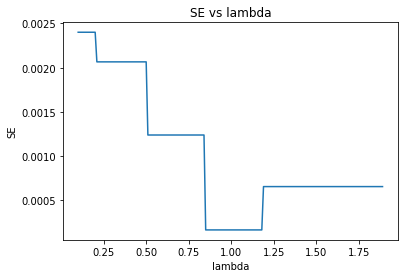
\includegraphics[scale=.5]{2}\\
      There are a few interesting things about this graph:
      \begin{itemize}
        \item The optimum lambda falls in a small window with SE $\approx$ 0. From this, one can conclude that $\lambda \in (.85, 1.18)$ are all equally valid. $\lambda=1$ is thus chosen for simplicity.
        \item The blocking structure of the graph occurs because of the discrete nature of the function being optimized. The inclusion of certain integrals in the final sum is a result of their indicator being nonzero, which is a binary decision based on lambda. When a new indicator "turns on" for a given lambda, the function jumps sharply to the new sum.
      \end{itemize}
      With $\lambda$ known, the original test can \textit{finally} be carried out. The likelihood ratio of $\vec X'$ is expressed:
      \begin{align*}
        \Lambda(\vec X') &= \frac{\sup_t \{P(\vec X' | p = t)P(p=t) \text{ s.t. } t \in [0, \frac{1}{2}]\}}{\sup_t \{P(\vec X' | p = t)P(p=t) \text{ s.t. } t \in (\frac{1}{2}, 1]\}}\\
        &= \frac{\binom{12}{9} .5^{12}}{\binom{12}{9} (\frac{9}{12})^9(\frac{3}{12})^3}\\
        &= \frac{.5^{12}}{(\frac{9}{12})^9(\frac{3}{12})^3}\\
        &\approx .208098\\
      \end{align*}
      Since $.2$ is less than $\lambda=1$, I \textbf{reject the null hypothesis!}

    \subsection*{Frequentist}
      Under a frequentist paradigm, the stated hypothesis test is equivalent to computing:
      \begin{itemize}
        \item[] $\mathbf{H_0}$: $p_0 = \frac{1}{2}$
        \item[] $\mathbf{H_A}$: $p_0 > \frac{1}{2}$
      \end{itemize}
      The generalized likelihood ratio, in this case, is written:
      $$\Lambda(x) = \frac{P(\vec X | H_0)}{\sup_t \{P(\vec X | H_A)\}} < \lambda$$
      Solving for $\lambda$
      \begin{align*}
        P \hella(\frac{P(\vec X | H_0)}{\sup_t \{P(\vec X | H_A)\}} < \lambda \hella | H_0 \hella) = \alpha\\
        P \hella(\frac{\binom{12}{r}(\frac 1 2)^{12}}{\binom{12}{r}(\frac{r}{12})^r(1-\frac{r}{12})^{12-r}} < \lambda \hella | H_0 \hella) = \alpha\\
        P \hella(\frac{(\frac 1 2)^{12}}{(\frac{r}{12})^r(1-\frac{r}{12})^{12-r}} < \lambda \hella | H_0 \hella) = \alpha\\
      \end{align*}
      \begin{align*}
        \sum_{\tilde r=0}^{12} \indicate \hella(\frac{(\frac 1 2)^{12}}{(\frac{\tilde r}{12})^{\tilde r}(1-\frac{\tilde r}{12})^{12-\tilde r}} < \lambda \hella)P(r = \tilde r | H_0) = \alpha\\
        \sum_{\tilde r=0}^{12} \indicate \hella(\frac{(\frac 1 2)^{12}}{(\frac{\tilde r}{12})^{\tilde r}(1-\frac{\tilde r}{12})^{12-\tilde r}} < \lambda \hella)\binom{12}{\tilde r}\bigg(\frac{1}{2}\bigg)^{12} = \alpha\\
      \end{align*}
      The above expression is annoying to solve analytically. However, it can also be solved as a root finding problem with grid search. Reexpressing the objective as:
      $$- \alpha + \sum_{\tilde r=0}^{12} \indicate \hella(\frac{(\frac 1 2)^{12}}{(\frac{\tilde r}{12})^{\tilde r}(1-\frac{\tilde r}{12})^{12-\tilde r}} < \lambda \hella)\binom{12}{\tilde r}\bigg(\frac{1}{2}\bigg)^{12} = 0$$
      The following graph follows from a grid search over $\lambda$ with significance to the 6th decimal place\\[6pt].
      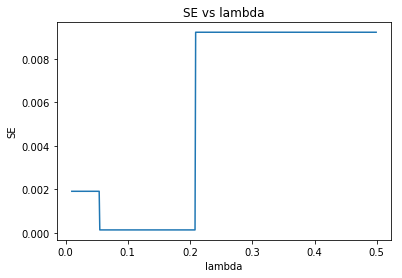
\includegraphics[scale=.5]{1}\\[6pt]
      There are a few interesting things about this graph:
      \begin{itemize}
        \item The optimum lambda falls in a small window with SE $\approx$ 0. From this, one can conclude that $\lambda \in [.055, .208098]$ are all equally valid.
        \item The blocking structure of the graph occurs because of the discrete nature of the function being optimized. The inclusion of certain terms in the final sum is a result of their indicator being nonzero, which is a binary decision based on lambda. When a new indicator "turns on" for a given lambda, the function jumps sharply to the new sum.
      \end{itemize}
      Now that $\lambda$ is known, the original test can be carried out. The likelihood ratio of $\vec X'$ has been calculated above, and is $\approx .208098$. Here a \textbf{very} interesting thing happens. The likelihood of the data is the \textbf{exact} endpoint of the interval of valid lambda. \textbf{PERO!} The likelihood ratio test, as constructed, rejects when the data likelihood is \textbf{strictly less than} the value of $\lambda$. Since $.208098$ is \textbf{not} strictly less than itself, I \textbf{fail to reject the null hypothesis!}\\[12pt]
      What the above shows is that the \textbf{VERY} subtle assumptions put forth in the analysis of data can have drastic implications for the conclusions drawn from the analysis.

    \section*{2}
      Consider a scenario where the true underlying distribution is a mixture of univariate gaussians where:
      \begin{itemize}
        \item $\mu_0 = -.25$; $\sigma_0 = 1$; $\pi_0 = .95$
        \item $\mu_1 = .25$; $\sigma_1 = 1$; $\pi_1 = .05$
        \item $n=128$
      \end{itemize}
      Additionally, consider a scenario where the training set has been intentionally class balanced before processing (i.e. it was enforced that $N_k = n_0 = n_1$). Furthermore, presume that a hypothetical analyst responsible for processing the data (let's call him Anton) did not know that the classes were pre-balanced. Anton decides he will estimate the mixing coefficients from the training data using $\hat \pi_k = \frac{n_k}{n}$ under the assumption that the data were collected in an iid manner. In this case, his Bayes plugin classfier (with the knowledge that the class variances are equal) collapses to the decision rule:
      \[g_a(x) =
        \begin{cases}
          0 & |x - \bar X_0| < |x - \bar X_1|\\
          1 & \text{else}\\
        \end{cases}
      \]
      We can compare this to an alternative classifier which has knowledge of the underlying mixing coefficients. Anton could have obtained the information about the skewed priors if he, perhaps, invested some time understanding the nature of the data generating process he was analyzing, instead of simply assuming iid collection. In this case, the liklihood funciton refers to a normal pdf with the given mean equal variances (estimated from the pooled sample variance under the assumption that the class variances are equal):
      \[g_b(x) =
        \begin{cases}
          0 & \mathcal L(x | \mu = \bar x_0, \sigma^2 = s_p^2).95 > \mathcal L(x | \mu = \bar x_1, \sigma^2=s_p^2).05\\
          1 & \text{else}\\
        \end{cases}
      \]
      A monte carlo simlation was performed to compare the accuracy of the classifier which assumes equal priors $g_a$, and a bayes plugin classifier which utilizes knowledge of the correct underlying priors $g_b$. Below is a histogram detailing the relative performance of the two algorithms over 100 monte carlo replications, with training set size $100$ and test set size $250$ :\\[6pt]
      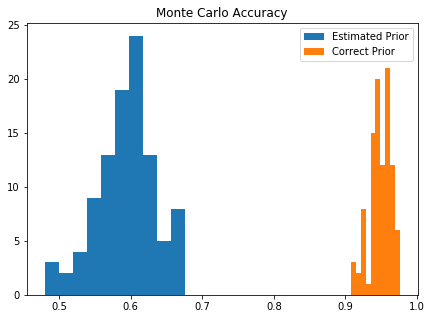
\includegraphics[scale=.5]{3}\\[6pt]
      Since both algorithms were trained on the same random train sets and tested on the same random test sets for each iteration, their accuracies can be considered paired. A Wilcoxin rank sums test was thus perfomred to test:
      \begin{itemize}
        \item[] $\mathbf{H_0}$ The distribution of accuracy for $g_a$ is the same for $g_b$
        \item[] $\mathbf{H_A}$ The distribution of accuracy for $g_a$ is \textbf{not} the same for $g_b$
      \end{itemize}
      This test results in a p value of $0$ \\[6pt]
      Thus, I \textbf{reject the null hypothesis!} There is evidence to suggest that the distributions of performance for $g_a$ and $g_b$ are different. Further, based on the distributions of the classifier results on this histogram, I infer that $g_a$ performs significantly worse than $g_b$ for classifying the data in question. For Anton, the assumption that the data were iid, along with its implication that $\hat \pi_k = \frac{n_k}{n}$ is a good estimate for $\pi_k$, causes \textbf{disasterous} results. Anton is promptly \textbf{fired} from his position.

    \section*{3}
      Anton has obtained a new position at a rival analytics firm. He is faced with a similar scenario, a two class gaussian classifcation where he knows that the variances both classes are equal. In this case:
      \begin{itemize}
        \item $\mu_0 = -1$; $\sigma_0 = 5$; $\pi_0 = .95$
        \item $\mu_1 = 1$; $\sigma_1 = 5$; $\pi_1 = .05$
      \end{itemize}
      Anton's new company, however, is much less well off than his old one, and thus only has the funds to collect $n=15$ data ponts.\\[6pt]
      Believing that he has learned from his mistake, Anton investigates the process that generates his data, and learns that $\pi_0 = .95$ and that $\pi_1 = .05$. He thus decides to \textbf{condition} his training set such that $N_k = n_k = \pi_k * n$ (i.e., he collects 95\% of the training examples from class 0 and 5\% from class 1.) His classifier for the data is as follows:
      \[g_c(x) =
        \begin{cases}
          0 & \mathcal L(x | \mu = \bar x_0).95 > \mathcal L(x | \mu = \bar x_1).05\\
          1 & \text{else}\\
        \end{cases}
      \]
      He decides to present this classifier to the company execs in comparison with a classifier that randomly selects the class prediction according to a coin flip. \textit{Certainly} his classifier will outperform random chance, right? The chart below compares Anton's classifier with the correct priors, trained on the  $N_k = n_k = \pi_k * n$ data, to a classifier that randomly assigns labels based on coin flips:\\[6pt]
      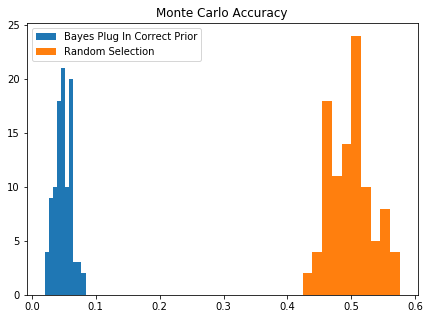
\includegraphics[scale=.5]{4}\\[6pt]
      Like the simulation from part 2, the clasifiers were "trained" on the same data (the random classifier ignores the training data), and tested on the same data, for each simulation. A Wilcoxin rank sum test was performed to test the hypothesis that:
      \begin{itemize}
        \item[] $\mathbf{H_0}$ The distribution of accuracy for $g_c$ is the same as random chance
        \item[] $\mathbf{H_A}$ The distribution of accuracy for $g_c$ is \textbf{not} the same as random chance
      \end{itemize}
      This test results in a p value of $0$\\[6pt]
      This, I \textbf{reject the null hypothesis!} There is evidence to suggest that $g_c$ and the random chance classifier have accuracies that arise from differnet distributions. Further, based on the histogram, I infer that Anton's classifier performs \textbf{worse} than random chance! Another \textbf{disasterous} result! Anton is promptly fired again.\\[12pt]

  The moral of the story here is that, no matter how clever you think you are, you are always at risk of making a huge error, even though your analysis seems sound based on what you know about the data. This is yet more evidence to validate the claim that \textbf{model selection is impossible, and free lunch is a lie}.




\end{document}
